Wie bereits im vorherigen \Abschnitt \ref{cha:2_Wellenausbreitung} angedeutet, besitzen elektromagnetische Felder in Abhängigkeit ihrer Frequenz unterschiedliche Eigenschaften, welche unterschiedliche Schirmungsmechanismen in Bezug auf die Abmessung der verwendeten Anordnung und der Art des Feldes notwendig machen. Da die Messungen im Rahmen dieser Arbeit im Fernfeld einer Antenne stattfinden sollen und auch der zu nutzende Freqeunzbereich mit $1\ldots$\SI{18}{\giga\hertz} deutlich über der Grenze von \SI{30}{\mega\hertz} liegt, ab der man nach~\cite{Design_of_shielded_enclosures} von der Ausbreitung ebener Wellen unabhängig von der Antennenbauart ausgegehen kann, soll sich die Betrachtung von Schirmungsmethoden auf das sogenannte elektromagnetische Wellenfeld beschränkten. Dies deckt sich mit der Einteilung elektromagnetischer Felder nach~\cite{Feldtheorie_Begriffe} und dem Richtwert für die Anwendung der Schirmungsmechanismen für Wellenfelder nach~\cite{EM_Schirmung}

\begin{equation}
    f > \frac{c_0}{d}
\end{equation}

mit einer Schirmabmessung $d$ im Bereich von \SI{1}{\meter} und Frequenzen $f$ im Bereich von $1\ldots$\SI{18}{\giga\hertz}.

%Induktion als charakteristisches Merkmal in diesem Anwednungsbreich



\subsection{Begriffe der Schirmdämpfung}\label{cha:2_sub_Begriff_der_Schirmdaempfung}

Um im Weiteren eine einheitliche Begriffsgrundlage vorauszusetzen, soll an dieser Stelle kurz auf die relevanten Begriffe der elektromagnetischen Strahlung und Schirmung eingegangen werden. Außerdem soll unter anderem die im Folgenden angewandte Konvention zur Darstellung von Bezugsgrößen logarithmierter Verhältnisse von Größen kurz eingeführt werden. 

\subsubsection{Pegelmaße}

Generell wird für die Darstellung von Verhältnissen elektrischer und magentischer Feldgrößen gern auf logarithmische Verhältnisse, sogenannte Pegel in Dezibel zurückgegriffen, was nicht nur den Vorteil eines großen Dynamikbereiches in der Darstellung hat, sondern auch verschiedene Rechnungen erleichtert. Unterschieden wird dabei zwischen relativen und bezogenen Pegeln. Relative Pegel, auch als Übertragungsmaße bezeichnet, stellen die Verhältnisse zweier Größen dar und dienen damit der Charakterisierung von Dämpfungen oder dem Ausdruck von Antennengewinnen. Für Feldgrößen $E$ ist der relative Pegel anders definiert~\cite{EM_Schirmung}

\begin{equation}
    E \si{\Dezibel} = 20 \cdot \log_{10} \left( \frac{E_1}{E_2} \right) = 20 \cdot \lg \left( \frac{E_1}{E_2} \right)
\end{equation}

als für Leistungen $P$

\begin{equation}
    P \si{\Dezibel} = 10 \cdot \lg \left( \frac{P_1}{P_2} \right) \; .
\end{equation}

Dies hat den Vorteil, dass bei der Rechnung mit Pegeln nicht auf die Art des vorliegenden Verhältnisses geachtet werden muss. Für ein intuitiveres Verständnis der Bedeutung bestimmter Pegel für das reale Großenverhältnis zweier Feldgrößen bzw. Leistungen sind in der \Tabelle\ref{tab:2_Relative_Pegel} gängige Pegel beispielhaft dargestellt.

\begin{table}
\renewcommand{\arraystretch}{\tablestretch}
\centering
\caption{Verschiedene relative Pegel mit zugehörigen Verhältnissen von Feldgrößen und Leistungen}
\vspace{\tablespace}
\begin{tabular}{l c c}
    \toprule
    Relativer Pegel $\left[\si{\Dezibel}\right]$ & Verhältnis von Feldgrößen & Verhältnis von Leistungen \\
    \midrule
    3   &   1,412   &   1,995   \\
    6   &   1,995   &   3,981   \\
    10  &   3,162   &   10      \\
    40  &   100     &   10.000  \\
    60  &   1000    &   1.000.000 \\
    80  &   10.000  &   $10^8$  \\
    100 &   100.000  &   $10^{10}$ \\
    \bottomrule
\end{tabular}
\label{tab:2_Relative_Pegel}
\end{table}

Bezogene Pegel beschreiben im Gegensatz dazu Absolutwerte einer Größe in Bezug auf einen Referenzwert, beispielsweise einen ungestörten Raumpunkt. Um wieder auf den ursprünglichen Wert der Größe schließen zu können, ist eine Angabe der Bezuggröße notwendig. Diese soll nach~\cite{IEC60027-3} wie folgt erfolgen: 

\begin{equation}
    P_{1 \si{\milli\watt}} = 10 \cdot \lg \left( \frac{P_1}{1 \si{\milli\watt}}\right) \si{\Dezibel} \; .
\end{equation}

Auf eine Kennzeichnung des Bezuges an der Einheit $\si{\Dezibel}$ soll ausdrücklich verzichtet werden, obwohl dies in der Literatur die vorherrschende Schreibweise ist. Für diese Arbeit soll jedoch die nach~\cite{IEC60027-3} korrekte Schreibweise $P_{1 \si{\milli\watt}} = 3 \si{\Dezibel}$ angewandt werden. 


\subsubsection{Schirmdämpfung}\label{cha:2_subsub_Schirmdaempfung}

Ein Schirm wird im Allgemeinen im Rahmen elektromagnetischer Anwendung dazu eingesetzt, Feldstärken im einem bestimmten Bereich innerhalb oder außerhalb des Schirms zu dämpfen. Nach dem Reziprozitätsgesetz ist es bei gleicher Feldverteilung, auch wenn diese in der Praxis oft nur bedingt gegeben ist~\cite{EMV-gerechtes_Geraetedesign}, dabei unerheblich, ob sich die Quelle des Feldes innerhalb oder außerhalb der Schirmgrenzen befindet~\cite{EM_Schirmung}. Die Schirmwirkung lässt sich mit dem Schirmfaktor $Q$, der die Feldstärke an einem Raumpunkt nach der Anwendung des Schirms (Index \glqq$1$\grqq) zur Feldstärke ohne Schirm (Index \glqq$0$\grqq) in Verhältnis setzt

\begin{align}
    Q_e = \frac{E_1}{E_0} \; \text{,}
\end{align}

beurteilen~\cite{EM_Schirmung}.
\par
\vspace{\linespace}
Die im Allgemeinen verursachte Phasenverschiebung durch den Schirm, macht $Q$ zu einer komplexen Größe~\cite{EM_Schirmung}. Da in den meisten Fällen jedoch vor allem der Betrag von Interesse ist, wird die Schirmdämpfung $a_s$ als Pegelmaß der Feldgrößenbeträge definiert:

\begin{align}
    a_e &= 20 \cdot \lg \left(\frac{\abs{E_0}}{\abs{E_1}}\right) = 20 \cdot \lg \frac{1}{\abs{Q_e}} \\
    a_m &= 20 \cdot \lg \left(\frac{\abs{H_0}}{\abs{H_1}}\right) = 20 \cdot \lg \frac{1}{\abs{Q_m}} \\
    a_s &= 10 \cdot \lg \left(\frac{\abs{P_0}}{\abs{P_1}}\right) \; \text{.}
\end{align}

Die Schirmdämpfung in Dezibel wird für ausgedehnte Schirme, aufgrund der teilweise starken Schwankungen zwischen einzelnen Raumpunkten hinsichtlich Feldverteilung und Frequenzen, nur als minimal erreichte Schirmdämpfung angegeben, da nur dieser Wert bspw. zur Charakterisierung der Schirmwirkung eines Gehäuses sinnvoll ist~\cite{EM_Schirmung}. Da nach der Definition der Schirmdämpfung die Feldgrößen einmal mit und einmal in Abwesenheit eines Schirmes gemessen werden muss und dies nicht zeitgleich erfolgen kann, bezeichnet man die Bestimmung der Schirmwirkung auch als Einfügungsmessung, da der Schirm im Verlauf der Messung zwischen Sende- und Empfangseinrichtung eingefügt wird. Auf die unterschiedlichen Messmethoden wird im \Abschnitt\ref{cha:2_Methoden_der_Schirmdaempfungsmessung} genauer eingegangen.


\subsection{Schirmung ebener Wellenfelder}\label{cha:2_sub_Schirmung_ebener_Wellenfelder}

Generell kann die Aussage getroffen werden, dass sich magnetostatische Gleichfelder von allen Feldarten am allerschwersten und nur mit hohen konstruktiven Aufwand abschirmen lassen~\cite{EM_Schirmung}. Vorteilhaft bei der Schirmung von Wellenfeldern ist im Gegensatz dazu die vorliegende Veränderung der magnetischen Feldstärke, welche elektrische Felder im Schirmmaterial induzieren können~\cite{Maxwell}


\begin{equation}
    \text{rot} \vec E= - \frac{\partial \vec B}{\partial t} \; \text{.}
    \label{eq:2_Induktionsgesetz}
\end{equation}

Mithilfe des Durchflutungsgesetzes~\cite{Maxwell}

\begin{equation}
    \text{rot} \vec H = \vec j_L + \frac{\partial \vec D}{\partial t}
    \label{eq:2_Durchflutungsgesetz}
\end{equation}

kann dies zur Schaffung eines wirksamen Schirmes genutzt werden. Für Frequenzen oberhalb von \SI{30}{\mega\hertz} und Feldquellen mit mehr als wenigen Zentimeter Abstand zum Schirm muss die Schirmdämpfung deshalb nicht für magnetische und elektrische Felder gesondert berechnet werden~\cite{Design_of_shielded_enclosures}. Dies gilt insbesondere für die Absorbtionsverluste im Material (siehe \Abschnitt\nameref{cha:2_subsub_Schirmungseffektivitaet}), die unabhängig vom Typ der Feldquelle sind~\cite{NASA_SP-3067}.   
\par 
\vspace{\linespace}
Die Wirkungsweise wird bei Betrachtung eines leitfähigen Materialblockes schnell deutlich. Bei Durchsetzung mit einem statischen Magnetfeld durchdringt dieses den Block vollständig und ohne jegliche Schirmung unter der Annahme $\mu = 1$. Handelt es sich bei dem Magnetfeld nun allerdings um ein Wechselfeld mit $f > 0$, so wird nach \Gleichung\eqref{eq:2_Induktionsgesetz} ein elektrisches Wirbelfeld um die magnetischen Flusslinien induziert~\cite{EM_Schirmung}. Im leitfähigen Material bilden sich daraufhin Wirbelströme aus, die nach \Gleichung\eqref{eq:2_Durchflutungsgesetz} ihrerseits ein Magnetfeld erzeugen, dass nach der Lenz'schen Regel seiner Ursache, also dem ursprünglichen, äußeren Magnetfeld entgegengerichtet ist und dieses durch Überlagerung abschwächt~\cite{EM_Schirmung}. Mit höherer Frequenz des Magnetfeldes und höherer Leitfähigkeit des Schirms steigt die Schirmwirkung des Materials aufgrund der besser fließenden Wirbelströme. Je höher die Frequenz, umso stärker verdichten sich die Magnetfeldlinien des äußeren und des Gegenfeldes am Rand des Materials, ebenso wie die Stromdichte~\cite{EM_Schirmung}. Der als Stromverdrängung bekannte Effekt führt bei hoher Frequenz so weit, dass die induzierten Ströme nur noch auf der äußeren Randschicht des Schirmmaterials fließen, was ebenfalls als Skineffekt bekannt ist. In diesem Falls wirkt nur die äußere Materialschicht dem anliegenden Feld entgegen, sodass die gleiche Schirmwirkung mit einer hohlen, leitfähigen Hülle erreicht werden kann, welche damit auch die einfachste Möglichkeit eines elektrodynamischen Schirmes darstellt. Die vorausgesetzte hohe Leitfähigkeit des Schirms hat außerdem den Vorteil, auch als Faraday'scher Käfig zu wirken und in hohem Maße elektrische Gleich- und Wechselfelder zu schirmen. Die erreichte Güte bei der Schirmung elektrischer Felder ist dabei bei gleichem Aufwand um Größenordnungen höher als die spezieller dielektrischer Schirme~\cite{EM_Schirmung}.
\par
\vspace{\linespace}
Für die beschriebene Wirkungsweise der Schirmung ist außerdem unerheblich, ob es sich bei dem Störfeld um ein quasitatisches oder ein ebenes Wellenfeld handelt~\cite{EM_Schirmung}. Ein Faraday'scher Käfig ist damit die effektivste Methode zur Schirmung elektrodynamischer Felder. Für Wellenfelder, deren Abmessung in der Größenordnung der Schirmausdehnung liegt, müssen jedoch Besonderheiten berücksichtigt werden, auf die im \Abschnitt\nameref{cha:2_subsub_Hohlraumresonanzen} eingegangen wird.  


\subsubsection{Eindringtiefe}\label{cha:2_subsub_Eindringtiefe}

Wie bereits beschrieben sind für die Eindringtiefe $\delta$, oder auch äuivalente Leitschichtdicke genannt, der Felder in des Schirmmaterial nicht nur die Materialparameter wie Leitfähigkeit $\sigma$ und Permeabilität $\mu$ entscheident, sondern auch die Frequenz des äußeren Feldes. Der Wert der Eindringtiefe ist für die vorliegende Situation nach~\cite{Taschenbuch_HF-Technik} definiert als

\begin{equation}
    \delta = \sqrt{\frac{1}{\pi f \mu \sigma}}
    \label{eq:2_Eindringtiefe}
\end{equation}

und gibt an, in welcher Entfernung von der Randschicht ein äußeres Feld um den Faktor $1/e \approx 37 \si{\percent}$ abgeschwächt wird~\cite{Taschenbuch_HF-Technik}. Innerhalb des Schirmmaterials entspricht der Feldverlauf dem einer gedämpften Welle~\cite{EM_Schirmung}. Für die richtige Dimensionierung eines elektrodynamischen Schirmes spielt die Eindringtiefe also eine wichtige Rolle, ebenso für eine geeignete Materialauswahl.


\subsubsection{Schirmungseffektivität}\label{cha:2_subsub_Schirmungseffektivitaet}

Für die Bestimmung der Effektivität eines Schirmes gegen eindrigende Strahlung ist jedoch nicht nur der Absorbtionsverlust durch Erzeugung von Wirbelfeldern, sondern auch der reflektierte Anteil der eintreffenden Welle (vergleiche \Abschnitt\ref{cha:2_sub_Reflektion}) entscheident. Nach~\cite{Problems_in_shielding_electronic_equiptment, NASA_SP-3067} ergibt sich die Schirmungseffektivität $S$ in Dezibel aus

\begin{equation}
    S_w \; \left[\text{dB}\right] = R_w \; \left[\text{dB}\right] + A_w \; \left[\text{dB}\right] + B_w \; \left[\text{dB}\right]
\end{equation}

mit dem Reflektionsverlust \acs{R_w}, der Absorbptionsdämpfung \acs{A_w} und dem Korrekturfaktor \acs{B_w} für Reflektionen innerhalb des Schirms bzw. beim Übergang der inneren Grenzflächen (vgl. \Abschnitt\ref{cha:2_sub_Verhalten_an_Grenzflächen}). Für $A_w > 15 \si{\Dezibel}$ kann \acs{B_w} jedoch vernachlässigt werden~\cite{NASA_SP-3067}. Für den Fall, dass die Feldquelle mehr als eine Wellenlänge $\lambda$ oder in einem Abstand von mindestens $d^2 / \lambda$, mit der größten Ausdehnung der Feldquelle $d$, vom Schirm entfernt positioniert ist, ist für die Bestimmung von \acs{R_w} nach~\cite{NASA_SP-3067} die Beziehung für ebene Wellen in jedem Fall ausreichend.  
\par
\vspace{\linespace}
Zur einfacheren Bestimmung der Summanden \acs{R_w} und \acs{A_w} kann auf Nomogramme zurückgegriffen werden. Somit kann für eine gegebene Frequenz der zu schirmenden Welle und ein ausgewähltes Material direkt der entsprechende Verlust beim Materialdurchgang abgelesen werden. Im \Anhang\ref{Anhang:Nomogramm_Reflektionsdaempfung} und \Anhang\ref{Anhang:Nomogramm_Absorptionsverlust} sind die Schaubilder nach~\cite{Simplified_shielding} dargestellt. 
\par
\vspace{\linespace}
Beispielhaft ergeben sich folgende Dämpfungen für \SI{2}{\milli\meter} starke Bleche aus Aluminium und Stahl bei \SI{100}{\mega\hertz} und \SI{10}{\giga\hertz}:


\begin{table}[h]
    \renewcommand{\arraystretch}{\tablestretch}
    \centering
    \caption[Ausgewählte Absorptions-, Reflektionsdämpfungen verschiedener Bleche]{Ausgewählte Absorptions-, Reflektionsdämpfungen verschiedener Bleche (\SI{2}{\milli\meter})}
    \vspace{\tablespace}
    \begin{tabular}{p{2cm} p{3cm} C{2.5cm} C{2.5cm}}
    \toprule
    Frequenz & Material & $R_w \; [\si{\Dezibel}]$ & $A_w \; [\si{\Dezibel}]$  \\
    \midrule
    \SI{100}{\mega\hertz} & Aluminium   &  86 &  >1000 \\
    \SI{10}{\giga\hertz} & Aluminium    &  66 &  >1000 \\
    \SI{100}{\mega\hertz} & Stahl       &  58 &  >1000 \\
    \SI{10}{\giga\hertz} & Stahl        &  38 &  >1000 \\
    \bottomrule
    \end{tabular}
    \label{tab:2_Beispielwerte_Schirmdaempfungen}
\end{table}

Wie leicht zu erkennen ist, nehmen die Absorptionsverluste im Material bei den betrachteten Frequenzen trotz der geringen Materialstärke bereits so hohe Werte an, dass praktisch davon ausgegangen werden kann, dass die Welle im Schirm vollständig ausgelöscht wird. Für Aluminium und andere \ac{NE-Metalle} ist dies durch die hohe Leitfähigkeit zu erklären (vgl. \Gleichung\eqref{eq:2_Eindringtiefe}), bei ferromagnetischen Materialien spielt die Permeabilität zusätzlich eine große Rolle für die Eindringtiefe elektromagnetischer Wellen in einen Schirm und damit die erreichbare Schirmdämpfung für eine gegebene Materialstärke. 
\par 
\vspace{\linespace}
Die höheren Reflektionsdämpfungen des Aluminiums sind auf die höhere Leitfähigkeit $\sigma$ im Vergleich zu Stahl zurückzuführen. Auch wenn diese für die Einfügungsdämpfung keinen nennenswerten Beitrag leisten, werden sie bei der Betrachtung von Hohlraumresonanzen innerhalb eines Schirmes relevant. 
\par
\vspace{\linespace}
Die theoretisch erreichbare Schirmdämpfung von mehr als \SI{1000}{\Dezibel} reduziert sich in der Praxis natürlich durch jegliche Öffnungen des Systems, durch die Störungen einkoppeln bzw. nach dem Reziprozitätsgesetz auskoppelt können. Für verschraubte Metallgehäuse kann bei sorgfältiger Platzierung der Verschraubungen eine Dämpfung von >\SI{100}{\Dezibel} erreicht werden~\cite{Design_of_shielded_enclosures}. Mit steigender Frequenz nimmt die praktisch erreichbare Schirmung ebenfalls ab, da die elektromagnetischen Wellen aufgrund der kürzeren Wellenlänge leichter über Spalte in das System gelangen können. Zu beachten ist auch, dass die theoretischen Schirmungseffektivitäten $S_w \geq 150 \si{\Dezibel}$ messtechnisch kaum oder nur mit großem Aufwand nachweisbar sind~\cite{EM_Schirmung}.
\par
\vspace{\linespace}
Zur Vermeidung von nichtlinearen Sättigungserscheinungen des Schirms werden in der Praxis des Weiteren häufig mehrschichtige Schirme eingesetzt, wobei die der Störung zugewandte Seite möglichst aus einem linearen Schirmmaterial mit niedriger Permeabilität bestehen sollte~\cite{EMV}. 



\subsubsection{Hohlwellenleiter}\label{cha:2_subsub_Hohlwellenleiter}
Das Phänomen der vollständigen Reflektion ebener Wellen an idealleitendes Flächen (vgl. \Abschnitt\ref{cha:2_sub_Reflektion}) legt eine Anwendung von Hohlkonstruktionen als Wellenleiter nahe. 
\par
\vspace{\linespace}
\begin{figure}
    \centering
    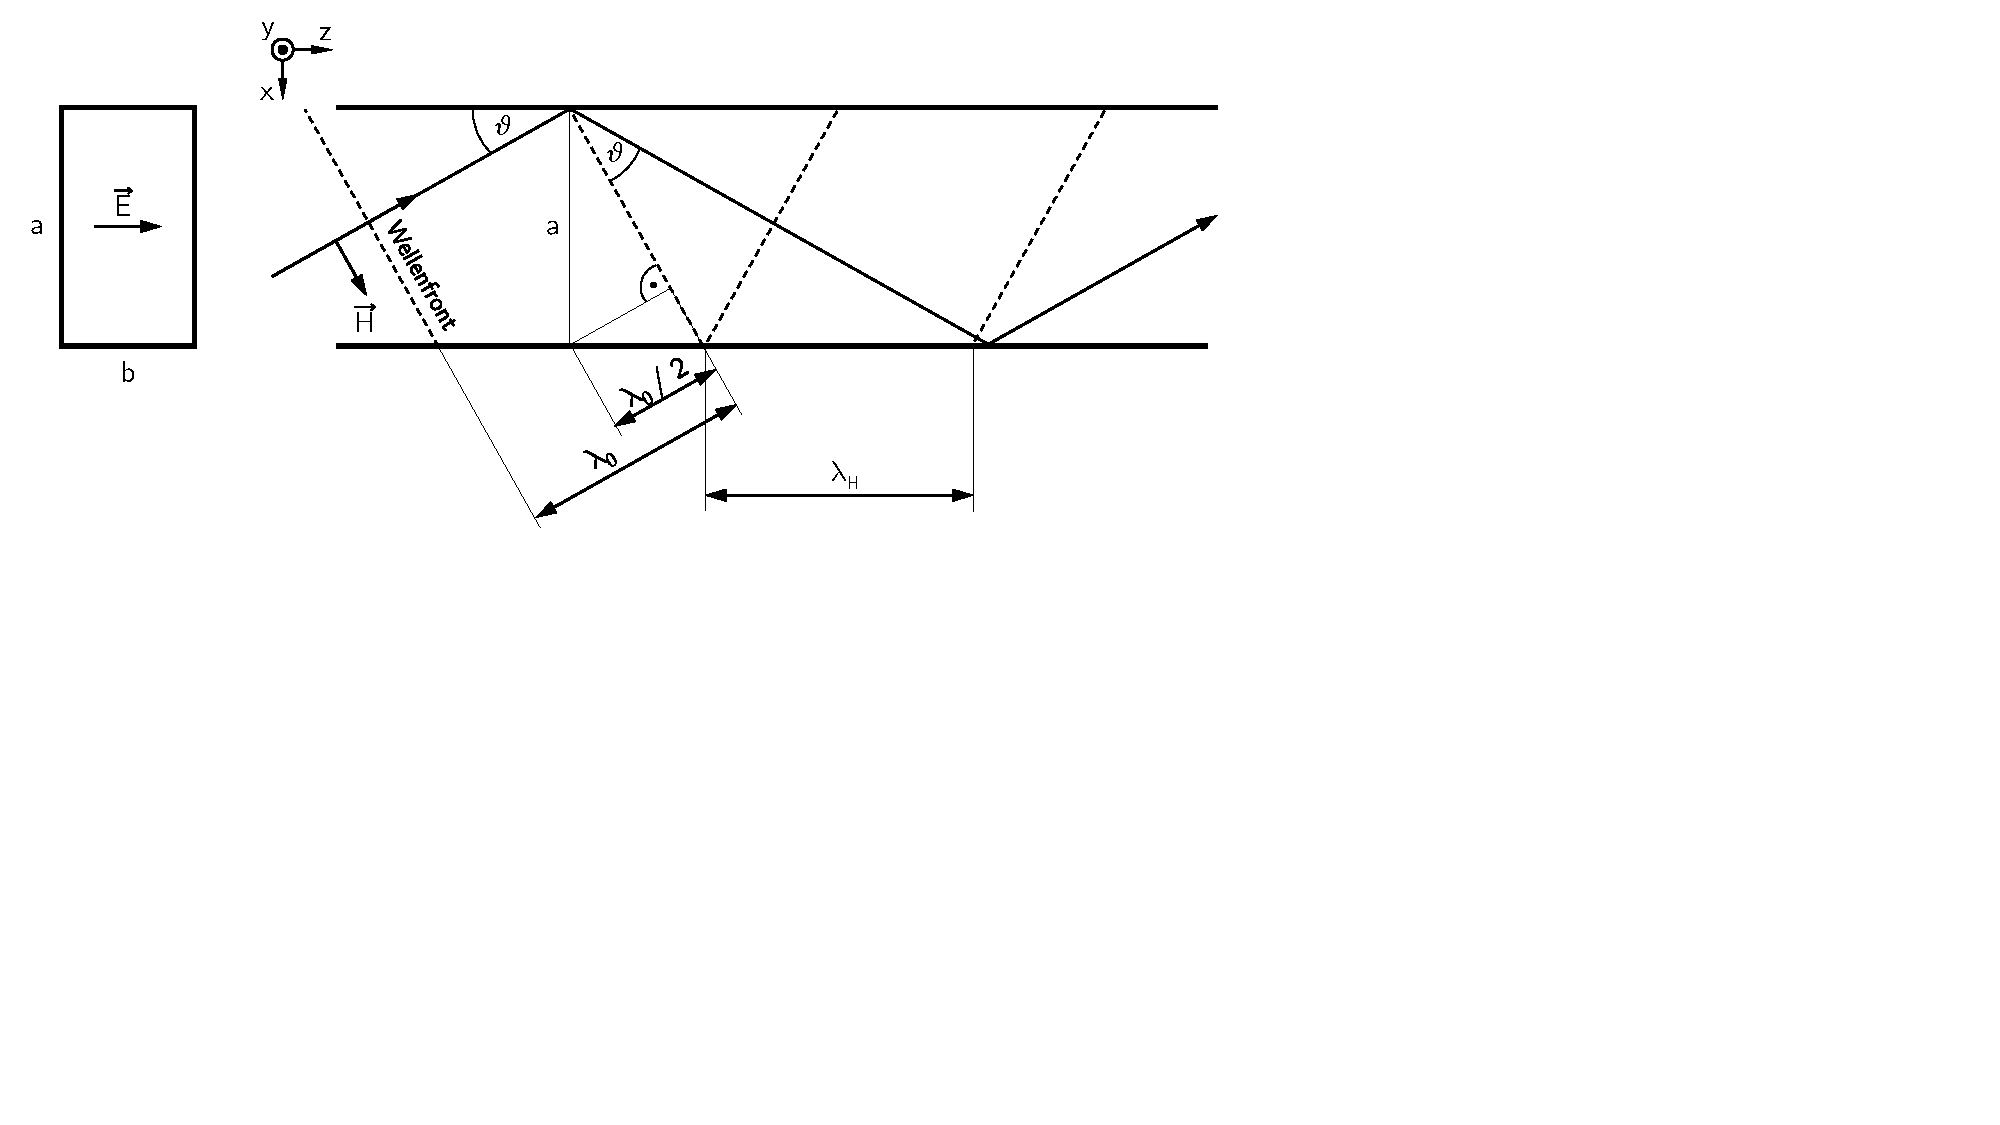
\includegraphics[scale = 1, trim = 0cm 10cm 13cm 0cm, clip, width=.8\textwidth]{Abbildungen/Kapitel2/Hohlwellenleiter.pdf}
    \caption{Schematische Darstellung eines Hohlwellenleiters im Schnitt nach~\cite{Taschenbuch_HF-Technik}}
    \label{fig:2_Hohlwellenleiter}
\end{figure}

Wird für eine ebene Welle, wie in \Abb\ref{fig:2_Hohlwellenleiter} dargestellt, ein E-Feldvektor parallel der Seitenwände mit einem zugehörigen H-Feldvektor angenommen, ist der Winkel $\vartheta$, unter dem die Ausbreitung der Welle stattfindet, nur von der längsten Seite des Hohlwellenleiters $a$ und der Freiraumwellenlänge $\lambda_0$ abhängig~\cite{Taschenbuch_HF-Technik}. Die Ausbreitungsbedingung ergibt sich aus dem Gangunterschied der reflektierten Wellenanteile, die sich möglichst konstruktiv überlagern sollten, d.h. einen Gangunterschied von $\lambda_0 / 2$ aufweisen sollten. Für das dargestellt Beispiel ergibt sich: 

\begin{equation}
    \sin{\vartheta} = \frac{n \cdot \lambda_0}{2 a} \; , \qquad n \in \mathbb{N}
\end{equation}
 
Mit $n=1$ wird dabei die Grundwelle beschrieben und mit $n>1$ die sogenannten höheren Wellentypen~\cite{Taschenbuch_HF-Technik}.
\par
\vspace{\linespace}
Die in  \Abb\ref{fig:2_Hohlwellenleiter} dargestellten gestrichelten Linien stellen die Ebenen konstanter Phase dar und deren Abstand ist die Hohlleiterwellenlänge $\lambda_H$ für die gilt~\cite{Taschenbuch_HF-Technik}:

\begin{equation}
    \lambda_H = \frac{\lambda_0}{\cos{\vartheta}}
\end{equation}

Mit sinkender Frequenz steigt also der Winkel $\vartheta$ und ebenfalls $\lambda_H$, bis für $\vartheta = 90\si{\degree}$ die Hohlleiterwellenlänge gegen unendlich geht. Das bedeutet es gibt eine untere, kritische Frequenz $f_k$, für die keine Wellenausbreitung im Hohlwellenleiter stattfinden kann. Dies kann für Öffnungen und Durchführungen in Schirme genutzt werden.
\par
\vspace{\linespace}
Zur Bestimmung der Grenzfrequenzen in verschiedenen Leiterquerschnitten müssen verschiedene Wellentypen unterschieden werden. H-Wellen (TE-Wellen, transversal-elektrisch) haben nur eine axiale magnetische Komponenten $H_z$ und E-Wellen (TM-Wellen, transversal-magnetisch) nur eine Längskomponente des elektrischen Feldes $E_z$, während die jeweils anderen axialen Komponenten Null sind~\cite{Taschenbuch_HF-Technik}. Die Kennzeichnung der Wellentypen geschieht über Indizes, die die Maxima in den unterschiedlichen Koordinantenrichtungen beschreiben. Die Grundwelle ist dann jeweils der Wellentyp, der innerhalb eines Querschnittes noch ausbreitungsfähig ist~\cite{Taschenbuch_HF-Technik}. In \Tabelle\ref{tab:2_Grenzwellenlaengen_Hohlleiter} sind die kritischen Wellenlängen für verschiedene Querschnitte mit den jeweiligen Grundwellentypen nach~\cite{Taschenbuch_HF-Technik} zusammengefasst.


\begin{table}[ht]
    \centering
    \renewcommand{\arraystretch}{\tablestretch}
    \caption{Kritische Wellenlängen für die Ausbreitung in verschiedenen Querschnitten mit Grundwellenform nach~\cite{Taschenbuch_HF-Technik}}\label{tab:2_Grenzwellenlaengen_Hohlleiter}
    \vspace{\tablespace}
    \begin{threeparttable}
    \begin{tabular}{p{5cm} p{4cm} C{3cm}}
    \toprule
        Hohlleiterquerschnitt & Anregung & $\lambda_k$ \\
    \midrule
        Rechteckquerschnitt & $H_{10}$-Mode & $2a$ \\
        Kreisquerschnitt    & $E_{01}$-Mode & $\approx 1,305 d$ \\
        Kreisquerschnitt    & $H_{11}$-Mode & $\approx 1,705 d$ \\
        Sechseckquerschnitt & $H_{10}$-Mode & $2a $\footnotemark[1] \\
    \bottomrule
    \end{tabular}
    \begin{tablenotes}
    \footnotesize
    \item[1] Näherung nach~\cite{EM_Schirmung} mit dem größten Abstand zweier Seiten $a$
    \end{tablenotes}
    \end{threeparttable}
\end{table}

\par
\vspace{\linespace}
Wellen mit $f < f_k$ erfahren innerhalb eines Hohlleiters mit der Länge $l$ eine Dämpfung~\cite{EM_Schirmung}:

\begin{align}
    S_{WL} \left[\si{\Dezibel}\right] &= 20\log_{10}\left(e^{\alpha\cdot l}\right)  \\
    \alpha &= \frac{2\pi}{\lambda_k} \sqrt{1-\left(\frac{\lambda_k}{\lambda_0}\right)^2} = \frac{2\pi f_k}{c_0} \sqrt{1-\left(\frac{f}{f_k}\right)^2} \qquad \text{für} \quad f < 0,8 f_k
\end{align}


\subsubsection{Hohlraumresonanzen}\label{cha:2_subsub_Hohlraumresonanzen}




